\section{Le membrane}
Dal punto di vista geometrico le membrane, siano esse biologiche o artificiali, possono essere schematizzate come pareti aventi spessore $\Delta x$ e fori cilindrici di raggio $R$ (\figurename~\ref{membrana}a) . Indicando con $V$ il \textit{volume}, è possibile definire un \textit{coefficiente di partizione} nel modo seguente:
\begin{equation}\label{coe_alpha}
	\alpha = \frac{V_{pori}}{V_{membrana}}= \frac{N_p \pi R^2 \Delta x}{A \Delta x} = n \pi R^2
\end{equation}
in cui $N_p$ è il numero dei pori, $A$ è l'area della superficie della membrana e $n=N_p/A$ è la densità superficiale dei pori. Si noti che per $\alpha=0$ la membrana è massiccia e priva di fori, mentre $\alpha=1$ identifica una membrana virtuale, praticamente inesistente. Il coefficiente di partizione rappresenta quindi la frazione di \textit{vuoto} della membrana.
\begin{figure}[htb]
	\centering
	\subfigure[]%
	{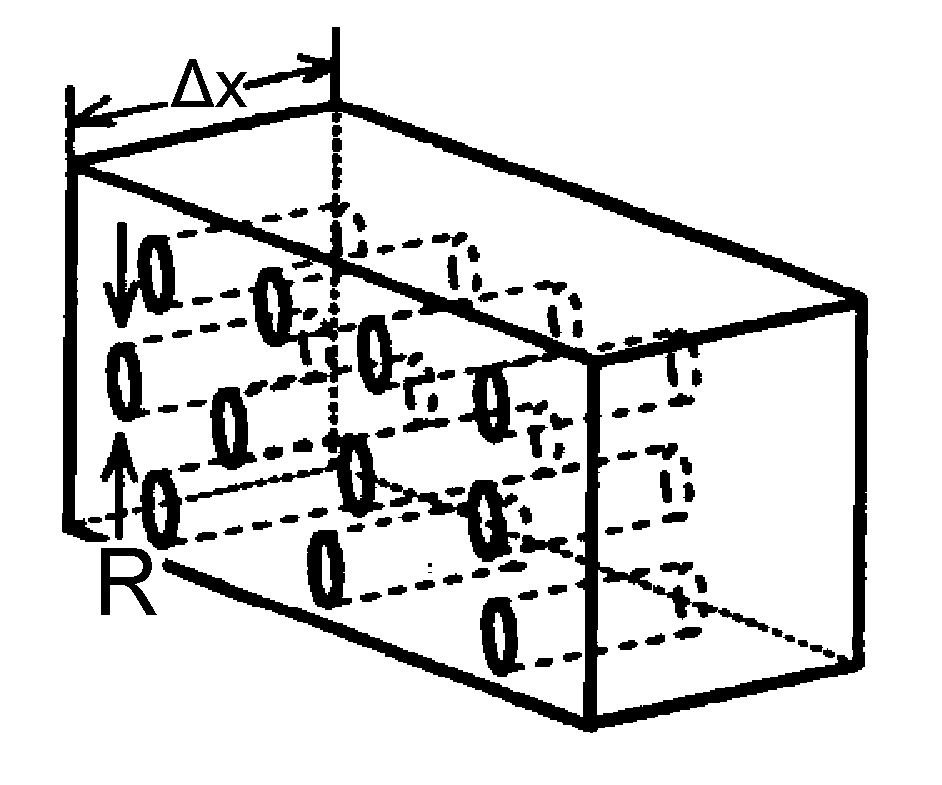
\includegraphics[width=0.3\textwidth]{immagini/membrana.eps}}\qquad
	\subfigure[]%
	{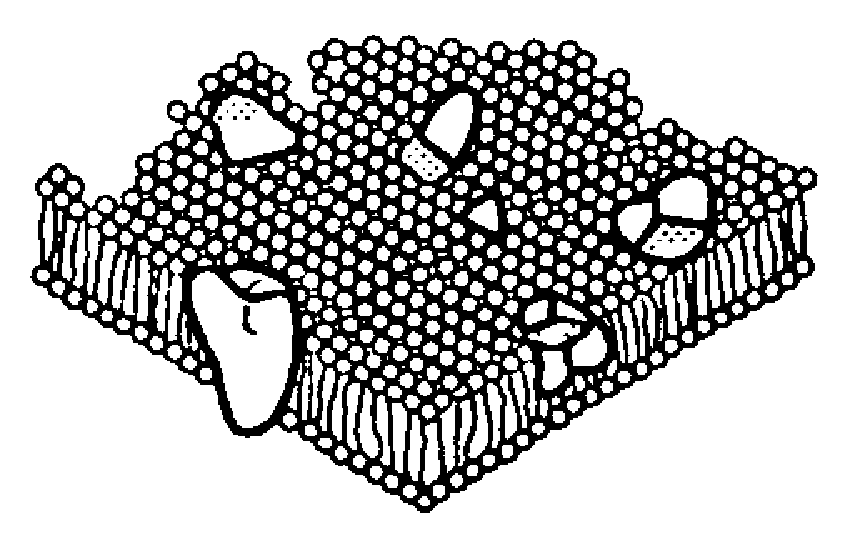
\includegraphics[width=0.45\textwidth]{immagini/membrana_cellulare.eps}}
		\caption{(a) Caratteristiche geometriche di una membrana. I fori hanno sezione media pari a $\pi R^2$ mentre $\Delta x$ rappresenta lo spessore medio della membrana. (b) Esempio di membrana biologica: doppio strato fosfolipidico con proteine di transmembrana come pori.}\label{membrana}
\end{figure}

Le membrane biologiche (\figurename~\ref{membrana}b) consentono il passaggio di sostanze tramite due meccanismi: fisici, o \textit{passivi}, e biochimici, o \textit{attivi}. Fra i meccanismi passivi vi sono la \textit{diffusione}, la \textit{convezione} e l'\textit{osmosi} e si tratta di fenomeni che avvengono spontaneamente fino al raggiungimento dell'equilibrio termodinamico. I meccanismi attivi richiedono invece l'uso di energia, solitamente fornita dall'idrolisi dell'ATP, in quanto si tratta di fenomeni di trasporto contro gradiente che tendono in generale a far diminuire lo stato entropico del sistema.
